% \addcontentsline{toc}{chapter}{Úvod}

% Jak již bylo zmíněno v úvodní částí, cílem této práce je vytvořit emulátor, emuluj
%
% Cílem praktické části je navrhnout a implementovat emulátor herní konzole NES tak, aby bylo dosaženo
% relativné funkční kompatibility s původním systémem. Návrh zahrnuje jak softwarovou realizaci
% architektonických prvků, tak návrh podpůrného hardwaru zajišťujícího interakci s okolím.

\chapter{Specifikace požadavků}

Před zahájením samotného návrhu hardwaru a implementace emulátoru bylo nezbytné definovat sadu
kritérií, která zajistí plynulý chod emulace a autentický uživatelský zážitek. Požadavky lze
rozdělit na systémové nároky a fyzická rozhraní zařízení.

\section{Software}

\begin{itemize}
    \item NES využíval NTSC jako standard pro analogové televizní vysílání, který pracoval se
        snímkovým kmitočtem 60~Hz. Emulátor musí generovat obraz stabilně při 60 snímcích za
        sekundu, aby nedocházelo k trhání obrazu.
    \item Emulator musí v reálném čase emulovat CPU, PPU a APU tak, aby byla zachována přesná časová
        souslednost mezi herní logikou, obrazem a zvukem.
    \item Z předchozích dvou bodů vychází, že mikrokontrolér musí být dostatečně výkonný aby stíhal
        emulovat, generovat obraz, zvuk a zpracovávat uživatelský vstup.
    \item Výsledný systém by měl obsahovat systémové menu, které umožní uživateli spouštět programy
        a konfigurovat běh celého systému.
    \item Aby se zachoval kód emulátoru udržovatelným a čitelným, systémové menu má být realizováno
        jako samostatný program, který bude schopen komunikovat s emulátorem, aby spouštět ostatní
        programy nebo konfigurovat emulátor. To je velice podobný koncepci BIOSu, což je program,
        určený pro načtení operačního systému a nízkoúrovňovou konfiguraci zařízení.
    \item Mikrokontrolér musí disponovat dostatkem paměti RAM pro uložení stavu emulátoru
        (stav jednotlivých komponentů, paměť programů, videopaměť) a dostatek pamětí (např. Flash)
        pro uložení samotného kódu firmwaru a obrazu BIOSu.
    \item Emulátor má být napsan v jazyce C bez přímých závislostí na specifickém hardwaru, což
        usnadňuje ladění na PC a případný budoucí port na jiné architektury.
    % \item Jelikož analogové vysílání už se nepoužívá, a jeho generace není jednoduchá, bude použito
    %     digitální video (většina moderních monitorů, displejů a televizí).1
    % \item Displej musí být rozšířený v domácnostech, a aby nedocházelo k trhání obrazu, musí mít
    %     dostatečně velkou rychlost komunikace, ale přitom takovou, kterou snese mikrokontrolér.
    % \item Ovládaní musí přesně mapovat standardní NES ovladač s minimální latencí.
    % \item Systém bude využívat SD kartu pro uchovávání a načítání programů, protože SD karty jsou
    %     rozšířené a velice dostupné, minimalistické a přenositelné, a jejích použití je lehčí než
    %     např. použití pevných disků nebo solid-state disků.
    % \item Systém musí mít uživatelsky jednoduchý způsob pro výběr programů a konfigurace zařízení.
    %     Může to být menu, které zobrazuje seznam programů uložených na SD kartě.
    % \item Firmware mikrokontroléru musí být snadno přeprogramovatelný uživatelem, nejlépe bez
    %     použití specializovaných programátorů, ideálně pomocí osobního počítače přes USB.
    % \item Kód samotného emulátoru musí být přenositelný a nezávislý na konkrétní platformě, což
    %     umožní jeho snadné testování na osobním počítači.
\end{itemize}

\section{Hardware}

\begin{itemize}
    \item Vzhledem k ústupu analogových technologií bude využit digitální standard HDMI, který je
        kompatibilní s většinou moderních monitorů a televizorů.
    \item Pro zajištění kvalitního poslechu bez nutnosti implementace komplexního digitálního audia
        přes HDMI bude zařízení vybaveno standardním 3,5mm Jack konektorem.
    \item Zařízení musí obsahovat dva porty pro připojení herních ovladačů pro podporu her
        více hráčů, podobně jako v originálním systému NES. Latence vstupu musí být minimální.
    \item Systém bude vybaven hlavním vypínačem (\textit{Power}) a dedikovaným tlačítkem
        \textit{Reset}, které umožní okamžitý návrat z programu do systémového menu (BIOSu).
    \item Pro ukládání programů a konfigurací bude využito rozhraní pro SD karty, které nabízí
        vysokou kapacitu při zachování jednoduché implementace a přenositelnosti dat.
    \item Napájení bude zajištěno přes standardní Barrel Jack konektor. Zařízení musí dále obsahovat
        USB rozhraní pro snadnou aktualizaci firmwaru uživatelem bez potřeby externího programátoru.
\end{itemize}

Na základě těchto požadavků byla zvolená vývojová deska \textbf{Raspberry~Pi~Pico~2}, řízená
mikrořadičem \textbf{RP2350}. Jedním z hlavních důvodů výběru této desky je její poměrně nízká cena
(v okamžik psaní této práce, průměrná cena této desky je 120 Kč), a mocný mikrořadič RP2350,
parametry kterého jsou popsány v datasheetu \cite{rp2350-datasheet}. Popis použitých periferií
RP2350 je možné najít v příloze G.

\begin{figure}[H]
    \centering
    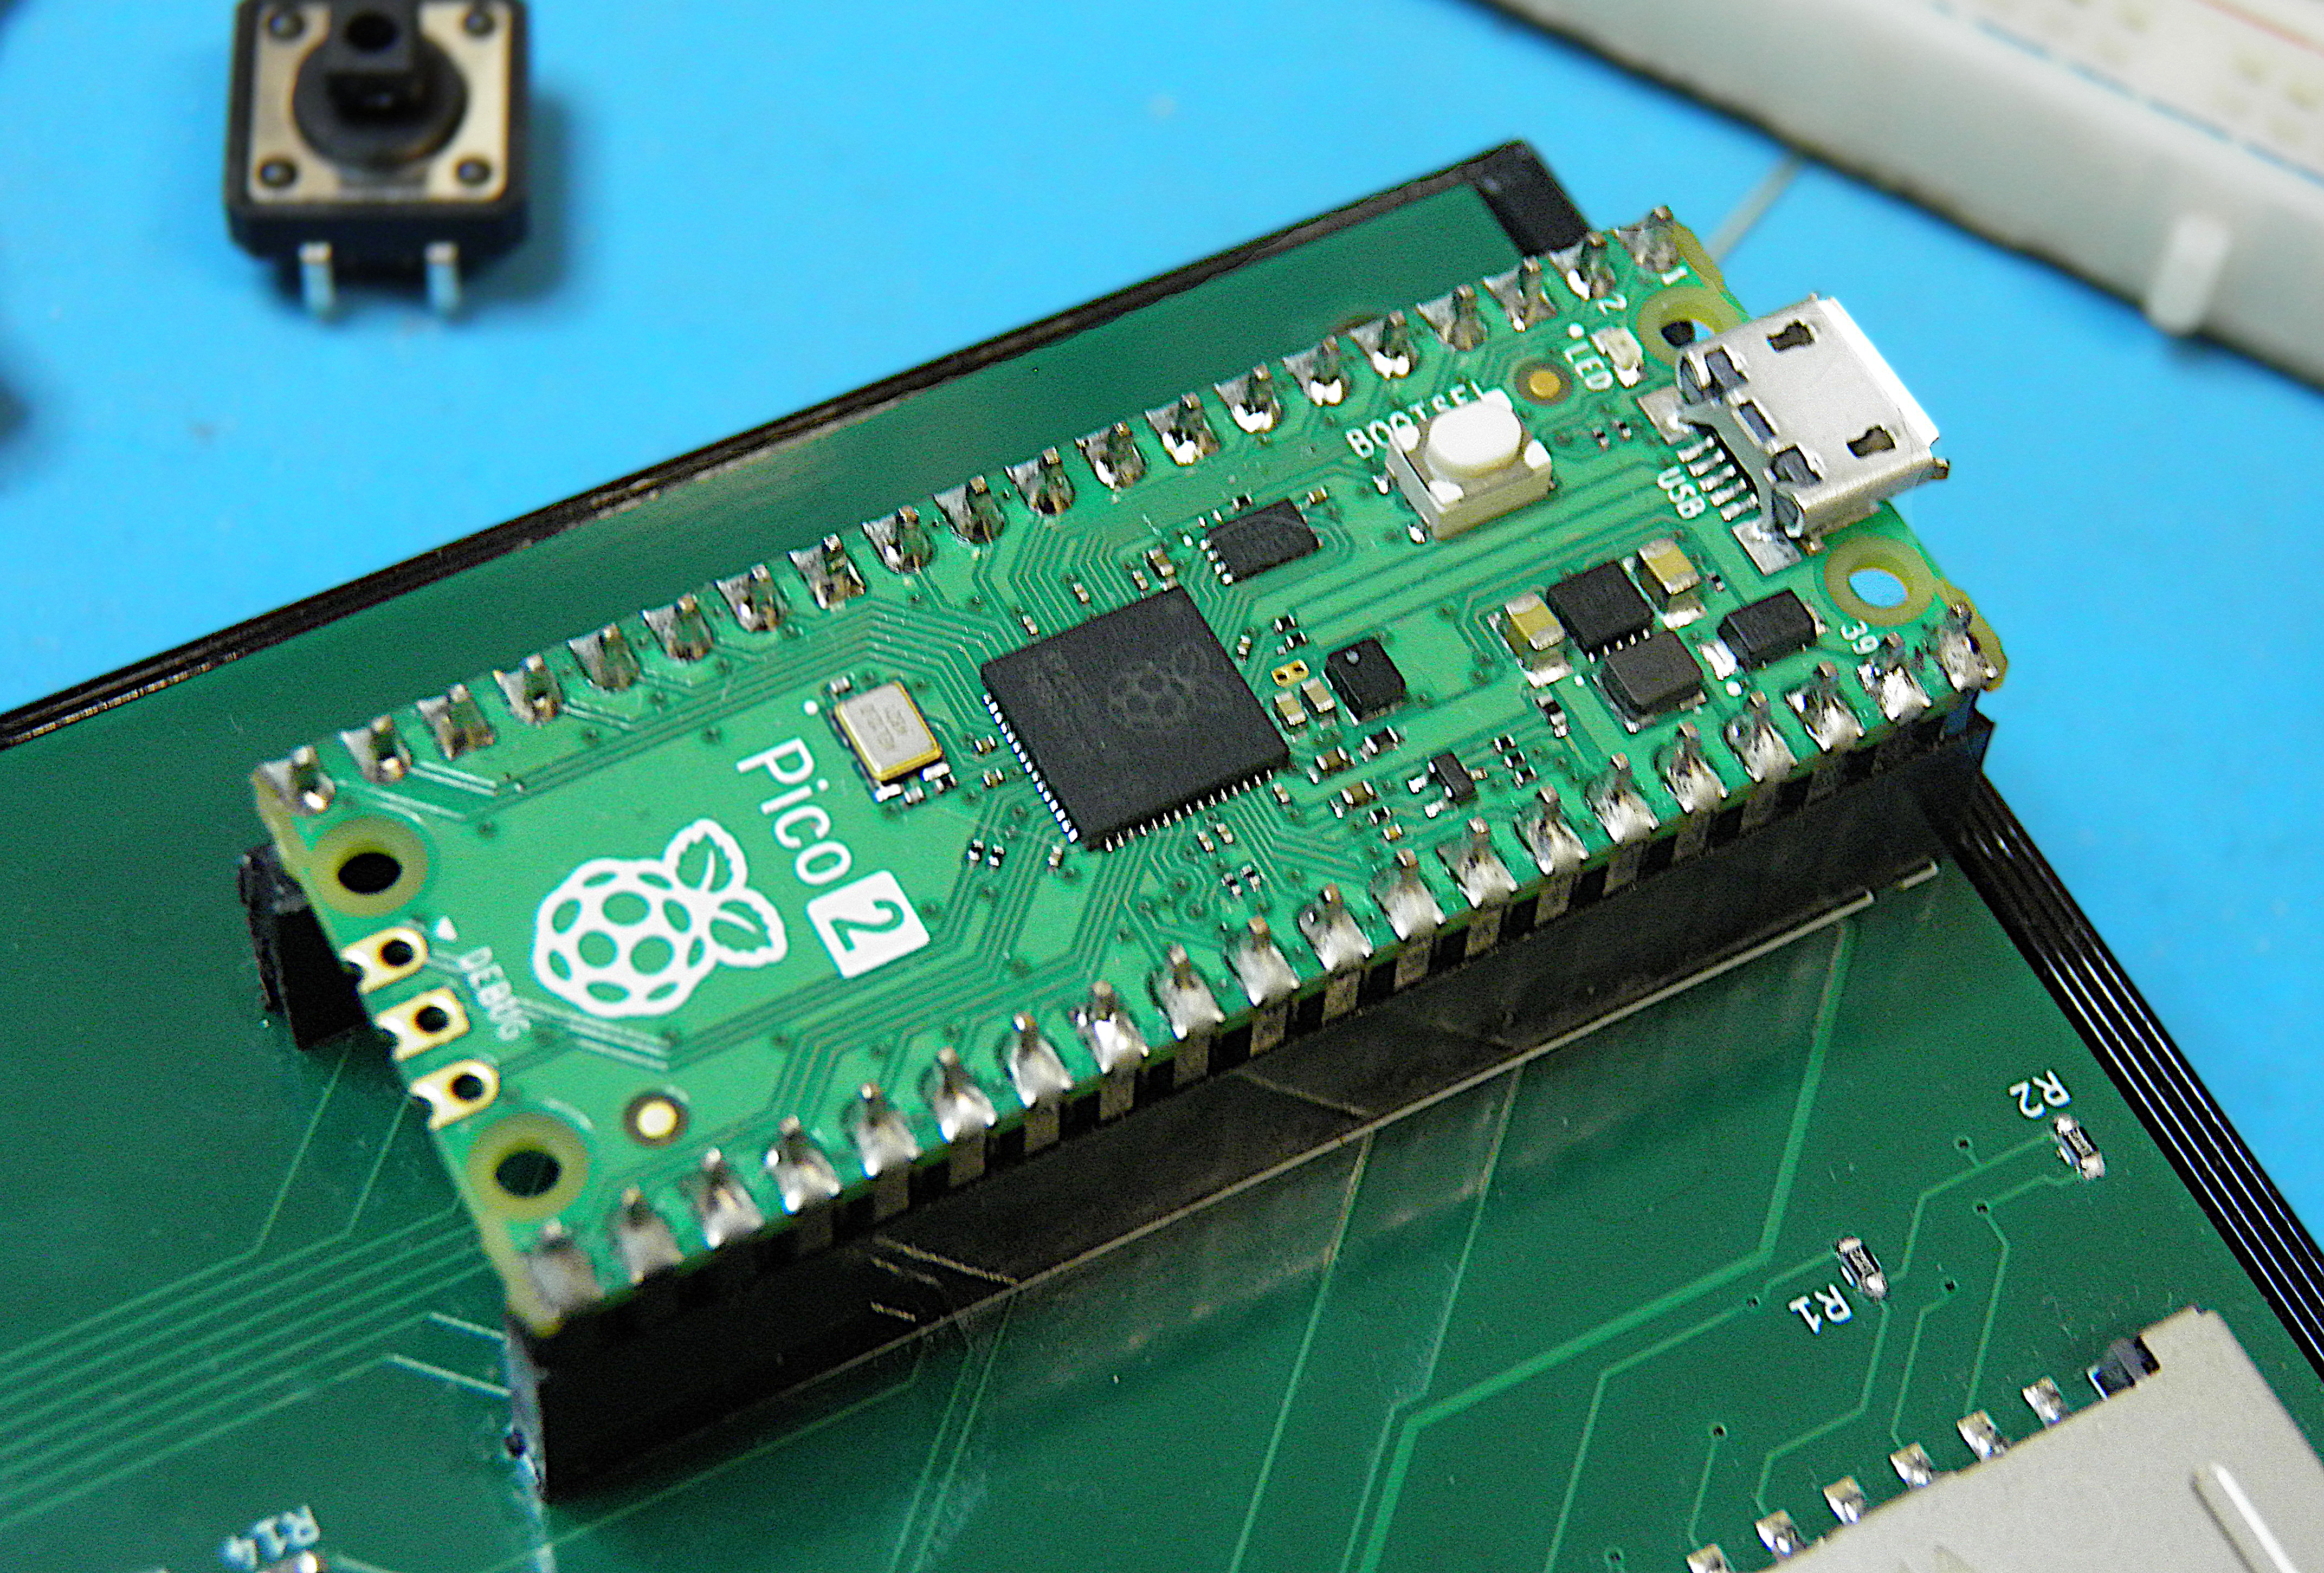
\includegraphics[height=8cm]{images/pico2.jpg}
    \caption{Vývojová deska Raspberry Pi Pico 2 s mikrořadičem RP2350.}
    \label{fig:pico2}
\end{figure}

\chapter{Architektura projektu}

Cely projekt je rozdělen do tři logických vrstev (viz
koncepční schéma \ref{fig:project_arch}):

\begin{figure}
    \centering
    \includesvg[width=\textwidth,height=\textheight,inkscapelatex=false]{images/fwkes_architecture.svg}
    \caption{Koncepční schéma architektury projektu, která je postavena na 3 vrstvách: emulátor,
        firmware a hardware.}
    \label{fig:project_arch}
\end{figure}

\begin{itemize}
    \item \textbf{Emulační vrstva} představuje bezprostředně samotnou emulaci CPU, PPU, APU,
        sběrnice, ovladačů a ROM obrazu programu. Jádro emulátoru je zcela abstraktní -- je
        nezávislé na platformě, a nemá povědomí o tom, na jakém koncovém zařízení běží. Tato vrstva
        mimo jiné obsahuje také jeden z hlavních přínosů našeho projektu -- komunikační linka FWX,
        což představuje most mezi emulovaným programem a emulátorem. FWX mapuje do emulované pamětí
        registry, diký kterým BIOS je schopen vyjít za rámec systému NES a komunikovat s emulátorem
        (například poslat požadavek o načtení programu).
    \item \textbf{Firmware} zajišťuje skutečnou realizaci výstupu a vstupu, a propojuje softwarovou
        část (emulátor) s hardwarovou částí. Tato vrstva předkládá požadavky emulátoru na reálné
        událostí a signály -- implementuje výstup obrazu pomocí DVI, generaci audio signálu,
        zpracovávání vstupu z tlačítek ovladačů, a komunikaci s SD kartou pro načtení programů.
    \item \textbf{Hardware} fyzicky propojuje mikrokontrolér s periferiemi a zajišťuje jeho správnou
        funkcí. Zahrnuje elektrické zapojení mikrokontroléru RP2350, napájení, ošetření signálových
        cest a integraci veškerých periferii a konektorů (HDMI, audio jack, porty pro ovladače, slot
        pro SD kartu a napájení).
\end{itemize}

Jednotlivé komponenty a technická řešení všech tří vrstev jsou detailně rozebrány v následujících
kapitolách.

\chapter{Struktura zdrojového kódu}

Při vývoji byl kladen důraz na modularitu a čisté oddělení platformově nezávislého jádra emulátoru
od specifické implementace pro cílový hardware (video, zvuk a vstup). Tato architektura umožňuje
snadné testování a ladění logiky emulace na osobním počítači (desktopový backend) před samotným
nasazením na mikrokontrolér.

Zdrojové soubory jsou organizovány do logických celků, které odpovídají funkčním blokům systému NES:

\begin{listing}[htbp]
\begin{minted}[fontsize=\small]{text}
docs/                  dokumentace
  soc/                 zdrojový kód tohoto skripta
include/
  fwkes/               .h soubory projektu
    cpu.h              deklarace CPU
    ppu.h              deklarace PPU
    ...
src/                   .c soubory projektu
  bios/                zdrojový kód BIOSu
  rp2350/              backend pro RP2350
  desktop/             backend pro PC
  cpu.c                implementace CPU
  ppu.c                implementace PPU
  ...
tests/                 testovací kód
third-party/           knihovny třetích stran
CMakeLists.txt         automatizace sestavování
\end{minted}
\caption*{Organizace zdrojového kódu projektu.}
\label{lst:src_code}
\end{listing}

Jelikož cílovou architekturou je mikrokontrolér RP2350, celý kód a struktura softwaru musí být
navržena tak, aby výsledný strojový kód byl dost rychlý a optimalizovaný na RP2350. Také neméně
důležité je efektivní správa pamětí a její úspora, jelikož interní SRAM paměť je pouhých 520 KB.
Jednotlivé techniky optimalizace budou popsány dále v textu.
